\documentclass[8pt]{beamer}
\usepackage{tikz}
\usepackage[utf8]{vietnam}
\usepackage{amsmath}
\usepackage{graphicx}
\usepackage{wrapfig}
\usepackage{hyperref}
\usetheme{Copenhagen}
\usecolortheme{dolphin}
\setbeamertemplate{navigation symbols}{}
\setbeamertemplate{headline}{}
\title[Chương 1: Quy trình ADC/DAC] %optional
{Chương 1: Quy trình ADC/DAC}
\subtitle{Xử lý tín hiệu số}
\author[Xử lý tín hiệu số] % (optional)
{Tín Vũ}
\date[VLC 2021] % (optional)
{tinvu1309@gmail.com}
\begin{document}
\frame{\titlepage}
\begin{frame}{Mục lục}
\tableofcontents
\end{frame}
\begin{frame}{Giới thiệu playlist}
\section{Giới thiệu playlist}
	\begin{itemize}
		\item Mình là Tín Vũ, hiện đang là sinh viên học tại Trường Đại học Công nghệ, Đại học Quốc gia Hà Nội. Mình tạo playlist video này để hỗ trợ các bạn học môn \textbf{Xử lý tín hiệu số}.
\item Khác với môn học tiên quyết \alert{Tín hiệu hệ thống} trước đó, bài giảng môn học này \textbf{hoàn toàn bám sát với đề cương và giáo trình nội bộ} của trường mình, nên các bạn trường khác cần phải lưu ý rất kĩ điều này.
\item Không chỉ dừng lại ở lý thuyết, playlist này \textbf{có bổ sung hướng dẫn lập trình cơ bản bằng GNU Octave/Matlab} để vẽ phổ tín hiệu, đáp ứng tần số và thiết kế bộ lọc.
\item Môn học này bao gồm \textbf{6 chương}, các chương đều liên quan rất chặt chẽ với nhau nên hãy học cẩn thận ngay từ \alert{Chương 0} để ôn thi cuối kì đỡ vất vả.
	\end{itemize}
\end{frame}
\begin{frame}{Tài liệu tham khảo}
\section{Tài liệu tham khảo}
\begin{itemize}
		\item Tài liệu tham khảo chính: Giáo trình Xử lý tín hiệu số (Nguyễn Linh Trung, Trần Đức Tân, Huỳnh Hữu Tuệ, ĐHCN, 2012).
		\item Tài liệu tham khảo phụ: Discrete-time Signal Processing (Alan V.Oppenheim, 2nd edition). 
	\end{itemize}
\end{frame}
\begin{frame}{Quy trình xử lý tín hiệu số}
\section{Quy trình xử lý tín hiệu số}
\begin{figure}[h]
			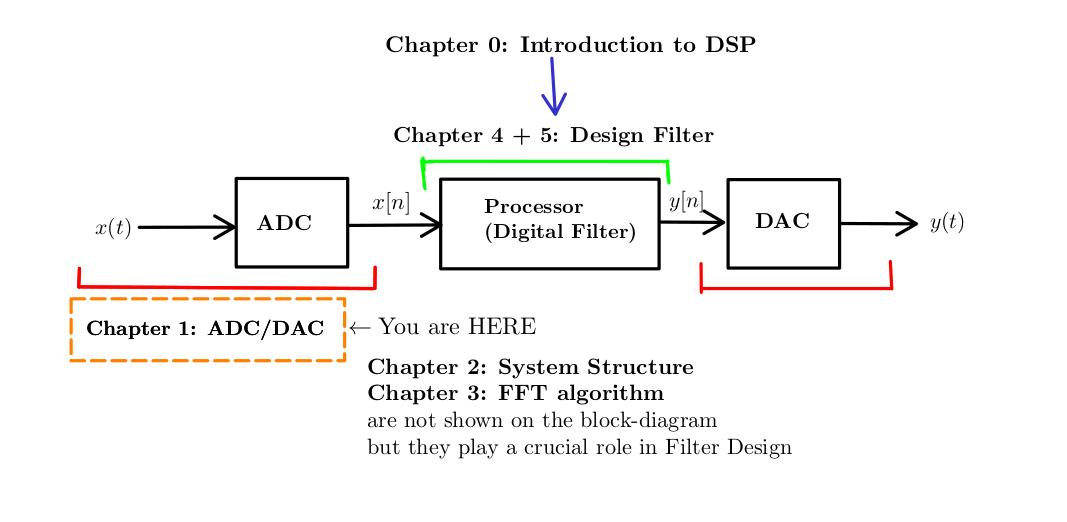
\includegraphics[width=1.1\textwidth]{1.jpg}
			\caption{DSP Learning Process}			\label{fig:re2}
		\end{figure}

\end{frame}
\begin{frame}{Quy trình ADC}
\section{Quy trình ADC}
\subsection{Quy trình lấy mẫu}
\begin{figure}[h]
			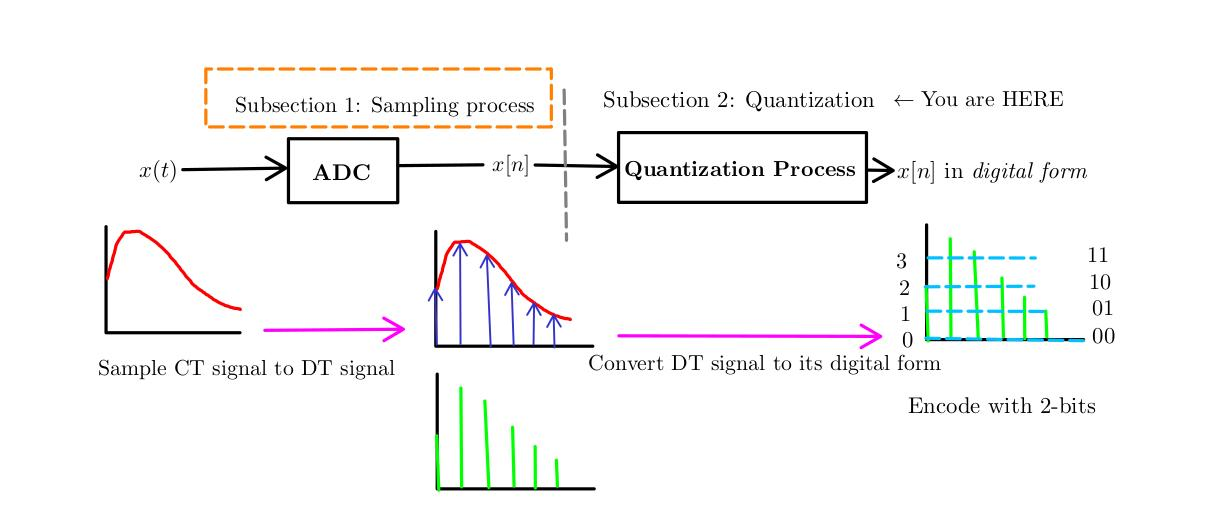
\includegraphics[width=1.1\textwidth]{2.jpg}
			\caption{ADC block diagram}			\label{fig:re3}
		\end{figure}


\end{frame}
\begin{frame}{Quy trình ADC}
\begin{itemize}
	\item[-] Quy trình lấy mẫu
\end{itemize}
Trong môn học tiên quyết \alert{Tín hiệu và hệ thống} trước, ta đã đề cập định tính về quy trình lấy mẫu để chuyển đổi tín hiệu liên tục thành tín hiệu rời rạc. Bây giờ, ta muốn tìm một mối liên hệ rất chặt chẽ về mặt toán học giữa tín hiệu $x(t)$ và $x[n]$ trong \textbf{miền thời gian} và \textbf{miền tần số}, và từ kết quả này ta sẽ xây dựng phương pháp chuyển đổi ngược tín hiệu rời rạc thành tín hiệu liên tục.
\begin{figure}[h]
			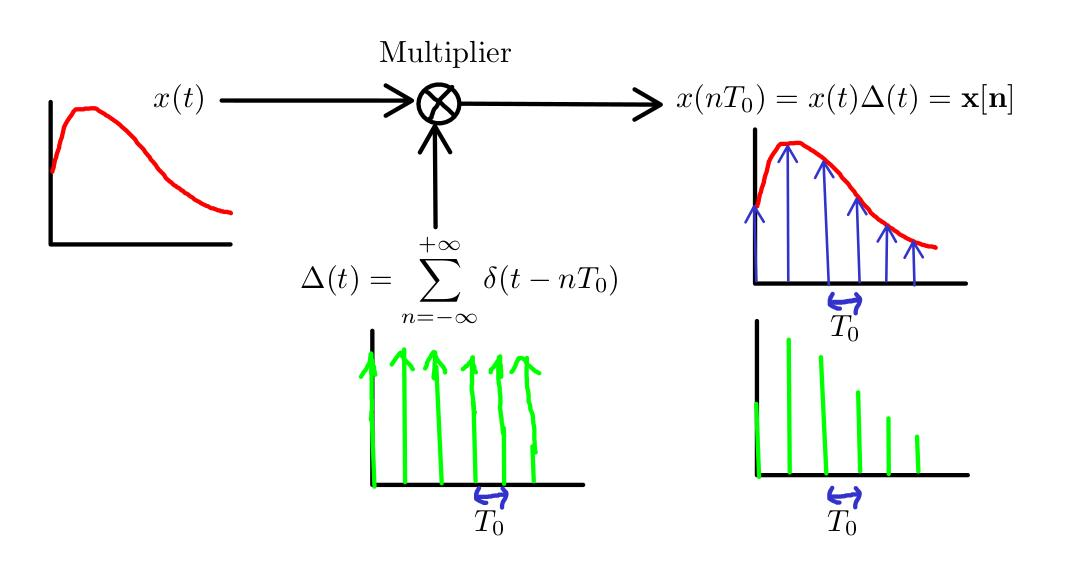
\includegraphics[width=0.8\textwidth]{3.jpg}
			\caption{Sampling process}			\label{fig:re4}
		\end{figure}

\end{frame}
\begin{frame}{Quy trình ADC}
	Trong môn học Xử lý tín hiệu số (từ giờ ta sẽ gọi tắt là DSP - Digital Signal Processing), các kí hiệu tần số \alert{ngược với môn Tín hiệu và hệ thống}, ta quy ước kí hiệu $\Omega$ cho tần số \textbf{liên tục} và $\omega$ cho tần số \textbf{rời rạc}. Từ mối liên hệ giữa $x(t)$ và $x[n]$, ta có:
\begin{equation*}
\begin{split}
	x[n]=x(nT_{0})=x(t)\Delta(t)=x(t)\sum_{n=-\infty}^{+\infty}\delta(t-nT_{0})
\end{split}
\end{equation*}
Dễ dàng nhận thấy $\Delta(t)$ có dạng \textbf{chuỗi Fourier liên tục (CTFS)}, ta thử tìm cách biểu diễn tín hiệu này về dạng chuỗi CTFS để phân tích trong miền tần số như sau:
$$\Delta(t)=\sum_{n=-\infty}^{+\infty}c_{n}e^{jn\Omega_{0}t}$$
$$c_{n}=\frac{1}{T_{0}}\int_{T_{0}}\Delta(t)e^{-jn\Omega_{0}t}=\frac{1}{T_{0}}\int_{-\frac{T_{0}}{2}}^{+\frac{T_{0}}{2}}\left[\sum_{n=-\infty}^{+\infty}\delta(t-nT_{0})\right]e^{-jn\Omega_{0}t}dt=\frac{1}{T_{0}}$$
Vậy ta thu được chuỗi CTFS của tín hiệu $\Delta(t)$: 
$$\Delta(t)=\frac{1}{T_{0}}\sum_{n=-\infty}^{+\infty}e^{jn\Omega_{0}t}$$
Ta xét biến đổi Fourier liên tục (CTFT) và tính chất \textbf{dịch trong miền tần số}:
\end{frame}
\end{document}
